  \label{introducao}
%Meu Mendeley tá com watch na pasta Dropbox da Edna
%Se eu achar artigo que eu vou usar e não está no Dropbox, enviar para a Edna

%Iniciando a escrita da Introducao. Lendo artigos sobre Requisitos de Privacidade a fim de encontrar questões de pesquisa que me guiem. Por isso, a introdução é crucial. Porém, já posso ir inserindo autores e artigos que serão utilizados no Cap 2.

%% Privacy Enhancing Techniques (PET)
%% Privacy by Design and by Default 
%% Privacy Impact Assessment (PIA)
%% Privacy Engineering
%% Threat Poker

%% Continuous Integration / Continuous Delivery (CI/CD) -- Como pode equipe ASD manter privacidade nisso
% Docker / GitLab

%Fichamentos dos artigos lidos encontram-se no fichamentos.tex

O que devo escrever na introdução? 9 parágrafos \todo[inline]{para saber você precisa ler os artigos e entender o assunto}

% Contextualização

% --- Engenharia de Requisitos : Elicitação de Requisitos. E ASD

A elicitação de requisitos é a atividade geralmente considerada como a etapa mais crucial no processo de Engenharia de Requisitos -- requisitos são a base para todos os produtos de software. As informações coletadas durante a elicitação de requisitos frequentemente têm que ser interpretadas, analisadas, modeladas e validadas antes que o engenheiro de requisitos possa se sentir confiante de que um conjunto completo de requisitos de um sistema foram obtidos \cite{EPICUREAN}.
 
Esta fase consiste em um conjunto de atividades que permitem descobrir, compreender e documentar quais são os motivos e objetivos que levam ao desenvolvimento de um sistema de software, envolvendo também a identificação dos requisitos que o sistema deve satisfazer a fim de atingir esses objetivos \cite{EPICUREAN}.
 
Atualmente, o mundo dos negócios é extremamente dinâmico e complexo, dado que as necessidades do mercado estão mudando rapidamente. Deste modo, os profissionais da área de Tecnologia da Informação enfrentam o desafio de reduzir o tempo em que um produto entra no mercado, fornecendo, ao mesmo tempo, produtos inovadores que agradem aos clientes. Além disso, o desafio de desenvolver produtos de software de acordo com requisitos que também estão mudando rapidamente.

O desenvolvimento ágil de software (ASD) promete benefícios como pontualidade na entrega e satisfação do cliente, portanto, tem como objetivo entregar valor ao negócio em pequenas iterações. Portanto, o processo de desenvolvimento é realizado de forma incremental e empírica, o que é uma vantagem, já que os requisitos de um sistema podem ser alterados imediatamente. 
 
Os requisitos a serem levantados podem variar de modificações a problemas e sistemas bem compreendidos (isto é, atualizações de software), a entendimentos nebulosos de novos problemas sendo automatizados, a requisitos relativamente sem restrições que estão abertos à inovação (por exemplo, o mercado de massa






% --- Design Thinking

% --- Privacidade

A evolução da Tecnologia da Informação está transformando tudo ao nosso redor, contribuindo para um aprimoramento na qualidade de vida. Sem embargo, essa evolução está também trazendo ameaças à direitos fundamentais de indivíduos como a questão de privacidade \cite{elshekeil2017gdpr}.

Existe um interesse do usuário que diverge no que diz respeito à privacidade e qualidade de serviço. Em outras palavras, se um usuário compartilha todos os dados com um serviço, este proporciona a melhor qualidade de serviço, porém colocando a privacidade do data subject em risco. Por outro lado, se o usuário não compartilha nenhum dado com o serviço, sua privacidade será garantida, mas os serviços proporcionados serão quase não existentes \cite{EPICUREAN}.

Lidar com a privacidade é uma atividade importante porque as violações de privacidade geram repercussões negativas e graves, tanto a imagem e reputação de empresas ou órgãos públicos, quanto financeiras e legais \cite{Gharib2016}.
% -- Inserir mais exemplos de Perda de dinheiro envolvendo brecha de privacidade por empresas

% ---- GDPR e LGDP

%%%%%%%%%%%%%%%%%%%%%%%%%%%%%%%%%%%%%%%%%%%%%%%%%%%%%%%%%%%%%%%%%%%%%%%%%%%%%%%%
\section{Problema de Pesquisa}
%%%%%%%%%%%%%%%%%%%%%%%%%%%%%%%%%%%%%%%%%%%%%%%%%%%%%%%%%%%%%%%%%%%%%%%%%%%%%%

1 a 2 paragrafos, nao sei como escrever

\todo[inline]{Aqui você deve abordar de maneira clara qual o problema que você pretende abordar no seu trabalho, descrevendo quais problemas existem e colocando as referencias de onde existe na literatura tal problema}

\todo[inline]{isso eu tentei responder em um artigo com a Angelica e até agora nenhum lugar aceitou so com um grupo focal, como vc faria isso?}
\begin{enumerate}[RQ.1:]

\item Quais as fases do Design Thinking são mais impactantes para a elicitação de requisitos de privacidade?

\item Quais as técnicas de Design Thinking podem ser utilizadas para facilitar a elicitação de requisitos de privacidade?

\item Quais as técnicas de elicitação de requisitos que são utilizadas atualmente para a elicitação de requisitos de privacidade?

\item As fases e ferramentas do Design Thinking podem motivar o desenvolvedor de software a identificar e tratar de forma mais eficaz os requisitos de privacidade?

\end{enumerate}

Para responder a RQ.1, RQ.2 and RQ.3 nós realizamos uma revisão de literatura para identificar as fases e técnicas do Design Thinking que são utilizadas na elicitação de requisitos de privacidade.

Para responder a RQ.4 nós realizamos um grupo focal com os desenvolvedores de software da ABIN. Nós exploramos questões relacionadas a .......


%%%%%%%%%%%%%%%%%%%%%%%%%%%%%%%%%%%%%%%%%%%%%%%%%%%%%%%%%%%%%%%%%%%%%%%%%%%%%%%%
\section{Justificativa}%
%%%%%%%%%%%%%%%%%%%%%%%%%%%%%%%%%%%%%%%%%%%%%%%%%%%%%%%%%%%%%%%%%%%%%%%%%%%%%%%%

3 a 4 paragrafos, nao sei como escrever. 

\todo[inline]{De acordo com o problema que você definiu, porque você irá pesquisar sobre? quais são os ganhos de pesquisar sobre? é justificar porque você irá pesquisar o problema}

Ele falou um monte de coisa dando embasamento pro ultimo paragrafo dele:
Poderia-se utilizar a abordagem proposta nesta pesquisa para propor a realização de um estudo de caso em um sistema que possibilitasse a implementação de algumas metodologias definidas na abordagem orientada à criatividade para preencher uma lacuna de pesquisa na identificação de indicadores de requisitos proposta no trabalho de Shalinka \cite{shalinka}, juntamente com a aferição dos resultados. Esse trabalho irá permitir uma validação objetiva dos ganhos alcançados com a aplicação da metodologia, porque não existe na literatura uma abordagem semelhante para a definição e priorização de indicadores.  

%%%%%%%%%%%%%%%%%%%%%%%%%%%%%%%%%%%%%%%%%%%%%%%%%%%%%%%%%%%%%%%%%%%%%%%%%%%%%%%%
\section{Objetivos}%
%%%%%%%%%%%%%%%%%%%%%%%%%%%%%%%%%%%%%%%%%%%%%%%%%%%%%%%%%%%%%%%%%%%%%%%%%%%%%%%%

\subsection{Objetivo Geral} 

1 paragrafo, nao sei como escrever. \todo[inline]{?????? - Qual é o objetivo do seu trabalho? O que você irá fazer?}

O objetivo geral deste trabalho é propor um modelo para definição e priorização de indicadores, utilizando mecanismos e ferramentas específicas para a tomada de decisão e com o foco no usuário final, como o \textit{Design Thinking} \cite{liedtka2018exploring}, \textit{Design Sprint} \cite{ferreira2019using} e o \textit{framework Cynefin} \cite{shalbafan2018decision}. Para isso, será necessário identificar os indicadores utilizados na literatura e na indústria e validá-los em um contexto real de desenvolvimento de software.

\subsection{Objetivos Específicos}
\label{obj}
%Esse aqui ta muito bom pra dar pequenas alteradas

Para atingir o objetivo geral deste trabalho,  os seguintes objetivos específicos foram definidos:

\begin{itemize}

    \item Realizar uma revisão de literatura para identificar os trabalhos que definem e priorizam indicadores, utilizando abordagens orientadas a tomada de decisão e com o foco no usuário, como o \textit{Design Thinking}, o \textit{Design Sprint}, o \textit{Cynefin Framework}, entre outros;
    
    \item Analisar as abordagens mais relevantes para serem utilizadas na implementação de um novo modelo para definir e priorizar indicadores com o foco no usuário, de forma eficiente;
    
    \item Propor uma nova abordagem para verificar, de uma forma mais precisa, quais indicadores, se melhorados, terão um impacto maior na eficiência do negócio \todo[inline]{verificar as virgulas -- propor uma nova abordagem mesmo????}. 
    
    \item Verificar a eficácia e a eficiência do modelo proposto através da comparação do resultado da entrega dos serviços de uma organização antes e depois dos indicadores serem priorizados e melhorados. 
    
    \item Realizar uma simulação para projetar os resultados das entregas dos serviços, caso outros indicadores fossem priorizados para serem melhorados. Se houver uma percepção maior na melhoria dos produtos e serviços, ao melhorar os indicadores que foram priorizados nos modelos em comparação com o resultado da simulação realizada com a melhoria de outros indicadores, então o modelo é válido e a escolha dos indicadores que foram melhorados foi adequada.
    
    \item Implementar e testar o modelo proposto em uma organização do mundo real;
    
    \item Validar o modelo proposto em um contexto real;
    
    \item Realizar caso necessário, ajustes no modelo proposto, incorporando melhorias a partir das observações/descobertas e realizadas na validação do modelo. 

\end{itemize}

%%%%%%%%%%%%%%%%%%%%%%%%%%%%%%%%%%%%%%%%%%%%%%%%%%%%%%%%%%%%%%%%%%%%%%%%%%%%%%%%
\section{Resultados Esperados}
%%%%%%%%%%%%%%%%%%%%%%%%%%%%%%%%%%%%%%%%%%%%%%%%%%%%%%%%%%%%%%%%%%%%%%%%%%%%%%%%

%Esse aqui ta muito bom pra dar pequenas alteradas

\begin{itemize}

\item Identificação das melhores práticas adotadas na academia e na indústria para a definição e priorização de indicadores orientada ao pensamento criativo;

\item Levantamento das soluções tecnológicas adotadas pelas organizações nos processos de gestão de indicadores;

\item Apresentação de um modelo de priorização e definição de indicadores centrado no usuário em que seja viável a sua implementação nas organizações que executam processos de desenvolvimento de soluções de TIC.

\end{itemize}

%%%%%%%%%%%%%%%%%%%%%%%%%%%%%%%%%%%%%%%%%%%%%%%%%%%%%%%%%%%%%%%%%%%%%%%%%%%%%%%%
\section{Metodologia de Pesquisa}
%%%%%%%%%%%%%%%%%%%%%%%%%%%%%%%%%%%%%%%%%%%%%%%%%%%%%%%%%%%%%%%%%%%%%%%%%%%%%%%%

3 a 4 paragrafos. Nao sei como escrever. Deixar mais pro final

\todo[inline]{eu coloquei dois livros ótimos no grupo para que possa ler e identificar, o frederico leu e conseguiu mapear para o trabalho dele.}
%%%%%%%%%%%%%%%%%%%%%%%%%%%%%%%%%%%%%%%%%%%%%%%%%%%%%%%%%%%%%%%%%%%%%%%%%%%%%%%%
\section{Estrutura do Trabalho}
%%%%%%%%%%%%%%%%%%%%%%%%%%%%%%%%%%%%%%%%%%%%%%%%%%%%%%%%%%%%%%%%%%%%%%%%%%%%%%%%

%Esse ta muito bom pra dar pequenas modificadas

Este trabalho está organizado em 5 capítulos, além deste, consistindo em:
\begin{itemize}

\item \textbf{Capítulo \ref{referencial}:} apresenta a fundamentação teórica necessária para o entendimento deste trabalho. Além disso, os trabalhos correlatos identificados na revisão de literatura são apresentados.

\item \textbf{Capítulo \ref{metodologia}:} apresenta a metodologia utilizada ao longo da elaboração deste trabalho.

%\item \textbf{Capítulo \ref{crono}:} apresenta uma perspectiva de atividades a serem realizadas para a finalização desse trabalho, assim como propõe o cronograma de execução de atividades. 

\item \textbf{Capítulo \ref{conclusoes}:} apresenta as principais conclusões deste trabalho e trata dos trabalhos futuros.
\end{itemize}

%%%%%%%%%%%%%%%%%%%%%%%%%%%%%%%%%%%%%%%%%%%%%%%%%%%%%%%%%
%Inicio tudo do Frederico

% Desde o surgimento das organizações orientadas por processo e projetos, observa-se a necessidade de se obter um grau de eficiência crescente no que diz respeito a utilidade e importância de determinados processos e projetos para o negócio das organizações \cite{paim2009gestao}.

% Tentou-se definir métricas e indicadores que cobrissem todas as atividades necessárias para o desenvolvimento e operação das atividades inerentes a organização, porém, ainda não se levava em conta a utilidade e adequação do indicador para o contexto do negócio. Somente com o aprimoramento das etapas que compõem a gestão por processos, que se começou a perceber a importância de se obter um entendimento claro sobre as necessidades do negócio \cite{paim2009gestao}.

% Alguns \textit{frameworks} e metodologias prescrevem e/ou sugerem um conjunto de passos a serem seguidos para alcançar, de forma eficiente e eficaz, uma definição clara das necessidades do negócio \cite{pressman} \cite{sommerville2007engenharia} \cite{teles2017extreme} \cite{fernandes2018requisitos} \cite{machado2018analise}. Entretanto, eles adotam uma estrutura mais tradicional, onde se avalia as necessidades do negócio com base em técnicas específicas para definição e priorização de indicadores \cite{pressman}. Ao longo da definição e priorização dos indicadores, se determina, dentro de um contexto pré-definido, quais são as necessidades e anseios dos gestores de negócio.

% Impulsionados pela necessidade de descobrir as reais necessidades do usuário, os profissionais de Tecnologia da Informação e Comunicação (TIC) não podem se limitar a definição e priorização de indicadores através de métodos que não levem em consideração a experiência do usuário e do negócio \cite{pressman}. Essa adequação deve abranger um  esforço concentrado em entender o usuário para buscar o que, de fato, o negócio necessita.

% Uma medida fundamental de sucesso para a definição e priorização de indicadores é o nível de envolvimento que a equipe de desenvolvimento assume com o usuário. Para manter o engajamento e confiança do usuário, o analista deve  buscar o pleno entendimento com o usuário através de outras abordagens, compartilhando e requerendo: conhecimento, experiências, visões e valores \cite{angelo}.

% Ao serem estimulados corretamente, os usuários podem externar necessidades que nem eles sabiam que poderiam existir. Esse fator reforça o sucesso de uma abordagem alternativa ao introduzir um mecanismo de definição e priorização de indicadores voltado ao pensamento criativo, empatia, ideação e criação de soluções inovadoras \cite{lockwood}.

% Alguns pesquisadores estão estabelecendo o foco das suas pesquisas em abordagens que busquem definir e priorizar indicadores de forma mais assertiva \cite{Ciriello}, \cite{lucassen}. De acordo com Ciriello et al. \cite{Ciriello} uma ferramenta bastante interessante, porém pouco utilizada na engenharia de software, é o \textit{Storytelling}. Essa ferramenta estabelece um entendimento comum entre as áreas técnicas, as áreas de negócio e os usuários, utilizada em conjunto com a técnica de prototipagem, se torna uma ferramenta eficiente para definir e priorizar indicadores \cite{Ciriello}. Uma outra proposta realizada por Lucassen et al. \cite{lucassen} para tornar a definição e priorização de indicadores mais assertiva, seria estabelecer um \textit{framework} para a definição das histórias de usuário. A abordagem define uma série de critérios a serem seguidos e uma ferramenta chamada AQUSA - \textit{Automatic Quality User Story Artisian} \cite{hotomski2019supporting}, utilizada para apoiar na definição de histórias de usuários mais eficazes, para que, através das histórias de usuário, possamos entender quais indicadores devem ser elaborados e, dos que já existem, quais devem ser priorizados para serem melhorados \cite{lucassen}. Esta abordagem parece ser mais adequada quando se opta por utilizar uma metodologia baseada em práticas ágeis.

% Ao utilizar esta nova abordagem, espera-se um ganho de eficiência nos processos e projetos cujos indicadores foram priorizados. O ganho de eficiência ocorreria por meio da diminuição de gastos com o retrabalho relacionado ao replanejamento, análise, desenvolvimento e implantação da solução. A redução dos custos consequentemente acarretaria também em uma redução do tempo para a entrega da solução para o demandante \cite{lucassen}. 

% Este trabalho apresenta uma revisão da literatura acerca de uma abordagem orientada ao pensamento criativo para a definição e priorização de indicadores, com o intuito de identificar na literatura como as empresas estão promovendo o desenvolvimento de uma abordagem mais assertiva para definir e priorizar quais indicadores serão otimizados, bem como quais são as melhores práticas adotadas para o processo de gestão de indicadores. Além disso, este trabalho apresenta o registro das soluções tecnológicas adotadas nos processos utilizados pelos casos de sucesso de acordo com a literatura e a indústria. A partir das soluções adotadas por empresas que adotam esta abordagem, este trabalho irá propor uma nova abordagem para definição e priorização de indicadores centrada no usuário e orientada ao pensamento criativo, baseado nas melhores práticas e ferramentas utilizadas nos casos de sucesso identificados.  

% %%%%%%%%%%%%%%%%%%%%%%%%%%%%%%%%%%%%%%%%%%%%%%%%%%%%%%%%%%%%%%%%%%%%%%%%%%%%%%%%
% \section{Problema de Pesquisa}
% %%%%%%%%%%%%%%%%%%%%%%%%%%%%%%%%%%%%%%%%%%%%%%%%%%%%%%%%%%%%%%%%%%%%%%%%%%%%%%

% A relevância da gestão de indicadores cresce e se torna mais impactante nos processos de negócio e nos projetos organizacionais à medida em que o processo evolui e se adapta às necessidades das organizações. Entender essas necessidades é vital para que os processos sejam executados de forma adequada e aderente aos princípios do negócio. Segundo Pressman \cite{pressman}, entender as reais necessidades do usuário é um ponto fundamental para o sucesso do desenvolvimento de qualquer solução. Assim, é importante refinar os métodos utilizados no processo de entendimento da necessidade do usuário final para que se possa prover uma solução que atenda as necessidades do usuário de forma adequada \cite{machado} \cite{pressman}.  É preciso definir um modelo que influencie e estimule os responsáveis pelos processos de negócio a expressar os seus problemas para que se possa entender claramente quais indicadores geram mais impacto nos processos de negócio. Dessa forma, é necessário utilizar ferramentas, como o \textit{Design Thinking} \cite{liedtka2018exploring}, \textit{Design Sprint} \cite{ferreira2019using} e o \textit{framework} Cynefin \cite{shalbafan2018decision}, que são capazes de capturar as necessidades do negócio e oferecer a identificação dos indicadores considerados de maior impacto na execução dos serviços.
	 

% %%%%%%%%%%%%%%%%%%%%%%%%%%%%%%%%%%%%%%%%%%%%%%%%%%%%%%%%%%%%%%%%%%%%%%%%%%%%%%%%
% \section{Justificativa}%
% %%%%%%%%%%%%%%%%%%%%%%%%%%%%%%%%%%%%%%%%%%%%%%%%%%%%%%%%%%%%%%%%%%%%%%%%%%%%%%%%

% Em virtude do valor agregado aos recursos de TIC nas organizações, torna-se necessário a identificação dos indicadores de avaliação da aceitação dos serviços e produtos fornecidos pela área de TIC, do ponto de vista do usuário. Os modelos atuais propõem um método que aborda a definição e priorização de indicadores através de métodos conceituais. Entretanto, tais modelos, por não haver um entendimento pleno das necessidades do usuário, tornam-se falhos quanto a objetividade e clareza. Se o processo de avaliação não utilizar indicadores que impossibilite avaliações ambíguas, os resultados podem ser diferentes, dependendo do ponto de vista do avaliador.

% A área de estudo da gestão de indicadores orientada ao pensamento criativo é uma área de pesquisa promissora, porém pouco estudada até o momento. Nguyen e Shanks \cite{nguyen} propuseram uma abordagem que define cinco grupos de criatividade: produto, processo, domínio, pessoas e contexto: 

% \begin{enumerate}
%     \item \textbf{Produto:} É frequentemente descrito como tendo as seguintes características principais: ter novidade, valor e ser surpreendente.
%         \begin{enumerate}
%             \item Ter novidade: Um produto criativo deve ser novo e original. Com base nos três níveis de criatividade, a novidade pode ser determinada nos níveis P, S ou H. Ideias relacionadas a novidade-P são ideias que parecem novas para o criador individual. As ideias relacionadas a novidade S ocorre como resultado de uma confluência do esforço individual e das culturas coletivas de domínios profissionais e grupos sociais; portanto, as ideias da novidade-S são ideias que são reconhecidas como novas e originais para o(s) grupo(s) profissional e social envolvido(s). As ideias da novidade-H parecem originais para todos \cite{nguyen}.
%             \item Ter valor: Um produto criativo também deve ser útil, ou seja, deve ser viável e eficaz na resolução de um problema. Nguyen e Shanks \cite{nguyen} descreveram o valor por meio da adequação, incluindo correção, bem como adequação do produto criativo ao contexto de uso.
%             \item Ser surpreendente: A surpresa é frequentemente associada a produtos criativos. Nguyen e Shanks \cite{nguyen} descreveram a surpresa como um impacto incomum e inesperado que pode nos chocar ou surpreender.
%         \end{enumerate}
%     \item \textbf{Processo:} O processo criativo pode ser definido como um processo interno de exploração e transformação de espaços conceituais em uma mente individual.
%     \item \textbf{Domínio:} O papel do domínio é fortemente reconhecido na visão sistêmica da criatividade. Primeiro, o domínio fornece um sistema simbólico e um corpo de conhecimento de uma disciplina. Segundo, o valor e a novidade do produto criativo devem ser definidos dentro de um domínio específico e o estado da arte desse domínio \cite{nguyen}.
%     \item \textbf{Pessoas:} As características pessoais comuns de indivíduos criativos podem ser categorizadas da seguinte forma: \textit{Traços} (original, articulador e fluente na geração de ideias), \textit{habilidades cognitivas} (Pensamento metafórico, sensibilidade de problemas e flexibilidade cognitiva) e \textit{estilos de resolução de problemas} (abordagem holística do pensamento, abordagem do pensamento lógico e experimentação) \cite{nguyen}.
%     \item \textbf{Contexto:} Os produtos criativos geralmente é o resultado do trabalho em equipe, feito de forma colaborativa. Os principais fatores que influenciam a criatividade da equipe podem ser classificados como cognitivos ou sociais. Os fatores cognitivos incluem habilidades de análise e síntese, habilidades processuais e organizacionais e conhecimento político. Fatores sociais individuais incluem a educação de cada membro da equipe, experiência de trabalho e cultura de fundo. Fatores sociais colaborativos incluem dinâmica de grupo e conflitos. \cite{nguyen} 
% \end{enumerate}

% Cada grupo de criatividade possui uma implicação direta com a atividade de elicitação de requisitos de software, conforme apresentado na Tabela \ref{tab:criatividadeengenhariarequisitos}. Hickey e Davis \cite{hickey} preocuparam em unificar os modelos de definição de indicadores por meio da fórmula: \[\sigma \left ( R_{i}S_{i}X(T) \right) \rightarrow T_{i} \subseteq T | se t \in T_{i}\] com a justificativa de destacar explicitamente o papel que o conhecimento do usuário desempenha na realização da seleção de indicadores a serem priorizados e de fornecer uma estrutura unificada para entender o papel da gestão de indicadores no desenvolvimento de software.

% \begin{table}[!htpb]
% 	\centering
% 	\caption{Implicações da pesquisa criativa para Engenharia de Requisitos (RE) \cite{nguyen}}
% 	\begin{center}
% 		\begin{tabular}{|p{2.4cm}|p{3.5cm}|p{4.5cm}|p{4.0cm}|}
% 			\hline
% 			\textbf{Elementos de Criatividade} & \textbf{Descrição} & \textbf{Implicações para ER} & \textbf{Pesquisa de Criatividade Relacionada com ER}\\
% 			\hline
% 			\multirow{4}{*}{1. Produto} 
% 			    & Novidade, valor e surpresa.
% 			    & Como novidade, surpresa e valor podem ser definidos e determinados na ER?
%                 & Integrar técnicas de criatividade para facilitar a descoberta de ideias e requisitos novos e úteis em ER.\\
%                 \hline
%             \multirow{4}{*}{2. Processo} 
% 			    & Inspiracionista, estruturalista e situacionista.
% 			    & Essas três visões não são mutuamente exclusivas. É necessária uma integração de visões para apoiar diferentes estilos e processos de pensamento criativo no ER.
%                 & Avaliando técnicas de criatividade no processo de ER.\\
%                 \hline
%             \multirow{4}{*}{3. Domínio} 
% 			    & Um debate entre visões gerais e específicas de domínio da criatividade continua.
% 			    & O ER envolve vários domínios. A pesquisa precisa esclarecer aspectos gerais e específicos do domínio da criatividade em ER. A educação em ER precisa abordar diferentes níveis de criatividade em geral e em domínios específicos, com estruturas educacionais apropriadas.
%                 & Estruturas educacionais foram propostas para apoiar a aprendizagem construtivista e experiencial para apoiar a criatividade nos domínios da ER e na área de problemas de negócios.\\
%                 \hline
%             \multirow{4}{*}{4. Pessoas} 
% 			    & Uma lista de características pessoais comuns identificadas e examinadas.
% 			    & Necessidade de identificar características pessoais comuns (características, habilidades cognitivas e abordagens de solução de problemas) possuídas por analistas de sistemas criativos.
%                 & Fatores individuais foram identificados através de estudos empíricos em um ambiente educacional.\\
%                 \hline
%             \multirow{4}{*}{5. Contexto} 
% 			    & Criatividade de nível S e processos sociais na produção, avaliação e adoção de produtos criativos.
% 			    & Necessidade de entender e apoiar o processo de equipe criativa colaborativa no ER.
%                 & Fatores organizacionais em diferentes níveis que influenciam a criatividade foram identificados por meio de um grupo focal e um estudo de caso em um ambiente educacional.\\
%                 \hline
% 		\end{tabular}
% 		\label{tab:criatividadeengenhariarequisitos}
% 	\end{center}
% \end{table} 

% Poderia-se utilizar a abordagem proposta nesta pesquisa para propor a realização de um estudo de caso em um sistema que possibilitasse a implementação de algumas metodologias definidas na abordagem orientada à criatividade para preencher uma lacuna de pesquisa na identificação de indicadores de requisitos proposta no trabalho de Shalinka \cite{shalinka}, juntamente com a aferição dos resultados. Esse trabalho irá permitir uma validação objetiva dos ganhos alcançados com a aplicação da metodologia, porque não existe na literatura uma abordagem semelhante para a definição e priorização de indicadores.  

% \section{Objetivos}

% \subsection{Objetivo Geral} 

% O objetivo geral deste trabalho é propor um modelo para definição e priorização de indicadores \todo[inline]{Frederico ainda não está claro que tipo de indicadores, por exemplo de Capabilities? de Gestao de Projetos? REquisitos? é preciso deixar claro porque existem muitos indicadores, com quais vc irá focar?}, utilizando mecanismos e ferramentas específicas para a tomada de decisão e com o foco no usuário final, como o \textit{Design Thinking} \cite{liedtka2018exploring}, \textit{Design Sprint} \cite{ferreira2019using} e o \textit{framework Cynefin} \cite{shalbafan2018decision}. Para isso, será necessário identificar os indicadores utilizados na literatura e na indústria e validá-los em um contexto real de desenvolvimento de software.

% \subsection{Objetivos Específicos}
% \label{obj}

% Para atingir o objetivo geral deste trabalho,  os seguintes objetivos específicos foram definidos:

% \begin{itemize}
%     \item Realizar uma revisão de literatura para identificar os trabalhos que definem e priorizam indicadores, utilizando abordagens orientadas a tomada de decisão e com o foco no usuário, como o \textit{Design Thinking}, o \textit{Design Sprint}, o \textit{Cynefin Framework}, entre outros;
    
%     \item Analisar as abordagens mais relevantes para serem utilizadas na implementação de um novo modelo para definir e priorizar indicadores com o foco no usuário, de forma eficiente;
    
%     \item Propor uma nova abordagem para verificar, de uma forma mais precisa, quais indicadores, se melhorados, terão um impacto maior na eficiência do negócio \todo[inline]{verificar as virgulas -- propor uma nova abordagem mesmo????}. 
    
%     \item Verificar a eficácia e a eficiência do modelo proposto através da comparação do resultado da entrega dos serviços de uma organização antes e depois dos indicadores serem priorizados e melhorados. 
    
%     \item Realizar uma simulação para projetar os resultados das entregas dos serviços, caso outros indicadores fossem priorizados para serem melhorados. Se houver uma percepção maior na melhoria dos produtos e serviços, ao melhorar os indicadores que foram priorizados nos modelos em comparação com o resultado da simulação realizada com a melhoria de outros indicadores, então o modelo é válido e a escolha dos indicadores que foram melhorados foi adequada.
    
%     \item Implementar e testar o modelo proposto em uma organização do mundo real;
    
%     \item Validar o modelo proposto em um contexto real;
    
%     \item Realizar caso necessário, ajustes no modelo proposto, incorporando melhorias a partir das observações/descobertas e realizadas na validação do modelo. 
    
% % Com relação a abordagem, foi corrigido. Com relação a proposição do modelo e validação do modelo, primeiro eu proponho um modelo e realizo o experimento. Se o resultado foi positivo, ou seja, se utilizando o modelo para priorizar indicadores eu tive um resultado melhor do que priorizando outros indicadores (validei o meu modelo), então o modelo foi validado e um contexto real. Se o resultado não foi melhor, o meu modelo possui falhas e eu preciso ajustá-lo de alguma forma. Por isso eu vejo que é importante tanto propor um modelo quanto validá-lo em um momento posterior, como objetivos específicos --- EDNA: Talvez isso aqui Frederico seja melhor na metodologia, porque os objetivos específicos são diretos: vou fazer isso - a forma como irei fazer seria na metodologia, vamos deixar aqui e na qualificação podemos ajustar o local}

% \todo[inline]{rever o título , está abordagem}
% \end{itemize}
% %%%%%%%%%%%%%%%%%%%%%%%%%%%%%%%%%%%%%%%%%%%%%%%%%%%%%%%%%%%%%%%%%%%%
% \section{Resultados Esperados}

% \begin{itemize}

% \item Identificação das melhores práticas adotadas na academia e na indústria para a definição e priorização de indicadores orientada ao pensamento criativo;

% \item Levantamento das soluções tecnológicas adotadas pelas organizações nos processos de gestão de indicadores;

% \item Apresentação de um modelo de priorização e definição de indicadores centrado no usuário em que seja viável a sua implementação nas organizações que executam processos de desenvolvimento de soluções de TIC.

% \end{itemize}

% \section{Metodologia de Pesquisa}

% A metodologia de pesquisa utilizada neste trabalho será a revisão da literatura em conjunto com um estudo de caso exploratório. A revisão da literatura objetiva reconhecer a unidade e a diversidade interpretativa existente no eixo temático em que se insere o problema em estudo, para ampliar, ramificar a análise interpretativa, bem como para compor as abstrações e sínteses que qualquer pesquisa requer colaborando para a coerência nas argumentações do pesquisador \cite{ferenhof2016desmistificando}. Ao final da revisão da literatura, espera-se obter um conjunto de indicadores que serão utilizados na aplicação do modelo proposto.

% O estudo de caso exploratório tem como finalidade proporcionar mais informações sobre o assunto a ser investigado, possibilitando sua definição e seu delineamento, isto é, facilitar a delimitação do tema da pesquisa; orientar a fixação dos objetivos e a formulação das hipóteses ou descobrir um novo tipo de enfoque para o assunto \cite{heidemann2016integraccao}.

% O estudo de caso exploratório será realizado com base no modelo proposto por Yin \cite{yin2017case}, que consiste em 6 passos:

% \begin{enumerate}
%     \item \textbf{Planejar o estudo de caso:} Identifica a situação relevante para a realização de um estudo de caso, comparado com outros métodos de pesquisa; compreende os benefícios de utilização de um estudo de caso; aborda as preocupações sobre a utilização de estudo de caso e, por fim, decide se deseja fazer um estudo de caso (Figura \ref{fig:processo_metodologia_pesquisa});
%     \item \textbf{Projetar o estudo de caso:} Identifica os casos e estabelece a lógica do seu estudo de caso; define o(s) caso(s) a ser estudado, desenvolve a teoria, as proposições e as questões relacionadas para orientar o estudo de caso e generalizar suas descobertas; identifica o desenho do estudo de caso (casos únicos ou múltiplos, holísticos ou incorporados) e testa o projeto com base em critérios pré-definidos para manter a qualidade de um estudo de caso (Figura \ref{fig:processo_metodologia_pesquisa});
%     \item \textbf{Preparar para coletar as evidências dos estudos de caso:} Aprimora as habilidades para realizar o estudo de caso; treina um estudo de caso específico; desenvolve o protocolo de estudo de caso; junto com a estratégia geral, leva em consideração algumas técnicas analíticas e aborda explicações e interpretações contrárias (Figura \ref{fig:processo_metodologia_pesquisa});
%     \item \textbf{Coletar as evidências dos estudos de caso:} Disponibiliza os dados por diferentes perspectivas; verifica os padrões, as ideias e os conceitos promissores e desenvolve uma estratégia analítica geral (Figura \ref{fig:processo_metodologia_pesquisa});
%     \item \textbf{Analisar as evidências dos estudos de caso:} Inicia com a definição das perguntas (por exemplo, as perguntas no seu protocolo de estudo de caso) e não com os dados. Inicie com uma pequena pergunta primeiro e depois identifique a evidência que a trata. Tire uma conclusão experimental com base no peso da evidência, perguntando também como você deve exibir a evidência para que as partes interessadas possam verificar sua avaliação (Figura \ref{fig:processo_metodologia_pesquisa});
%     \item \textbf{Compartilhar os estudos de caso:} Define audiência, seja para composições escritas ou orais; desenvolve materiais textuais e visuais; exibe evidência suficiente para o leitor chegar as suas próprias conclusões e revisa e recompõe até que a pesquisa esteja adequada e bem estruturada (Figura \ref{fig:processo_metodologia_pesquisa}).
    
% \end{enumerate}

% Para o desenvolvimento do estudo de caso exploratório, será utilizado um ambiente simulado de uma organização que não possui um mecanismo eficaz para definir e priorizar indicadores, e posteriormente em um ambiente real, com empresas de Brasília que entendam que a Tecnologia da Informação e Comunicação (TIC) é parte da sua visão estratégica. O desempenho da metodologia estudada e do modelo proposto serão mensurados a partir dos serviços fornecidos e produtos gerados pela TIC, previstos no Plano Estratégico de TIC (PETIC), em função das necessidades definidas pelo negócio e previstas no Plano Estratégico Institucional (PEI) das organizações. A Figura \ref{fig:processo_metodologia_pesquisa} representa o processo de execução da metodologia adotada:

% \begin{figure}[htb!]
% \centering
% 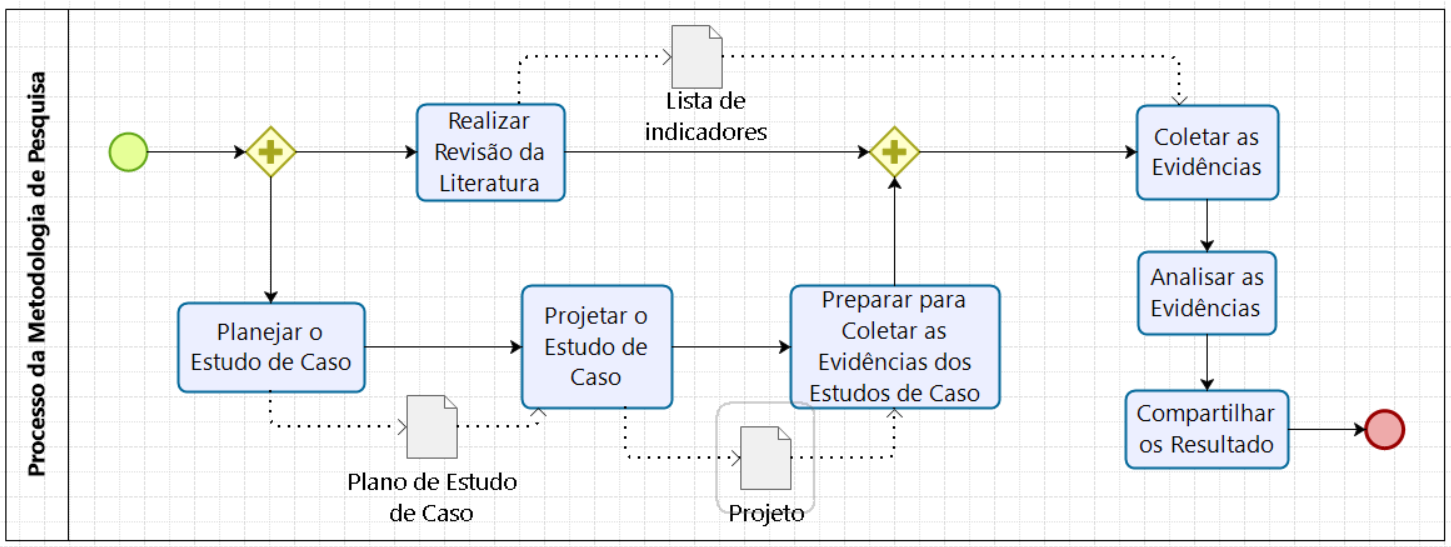
\includegraphics[width=1.0\textwidth]{img/processo_metodologia_pesquisa.png}
% \caption{Processo de execução da metodologia de pesquisa}
% \label{fig:processo_metodologia_pesquisa}
% \end{figure}
    
% \section{Estrutura do Trabalho}

% Este trabalho está organizado em 5 capítulos, além deste, consistindo em:
% \begin{itemize}

% \item \textbf{Capítulo \ref{embasamento}:} apresenta a fundamentação teórica necessária para o entendimento deste trabalho. Além disso, os trabalhos correlatos identificados na revisão de literatura são apresentados.

% \item \textbf{Capítulo \ref{modelo}:} propõe um modelo para a gestão de indicadores orientada ao pensamento criativo que possa contribuir com as organizações na priorização de seus indicadores. 

% \item \textbf{Capítulo \ref{crono}:} apresenta uma perspectiva de atividades a serem realizadas para a finalização desse trabalho, assim como propõe o cronograma de execução de atividades. 

% \item \textbf{Capítulo \ref{conclusoes}:} apresenta as principais conclusões deste trabalho e trata dos trabalhos futuros.
% \end{itemize}




